\chapter{Pengembangan Dan Pengujian}

\par Pada Tugas Akhir ini, perangkat lunak yang dikembangan berupa sistem manajemen kompetisi, \textit{autograder} dan program antar muka pengguna.  Sistem manajemen kompetisi di\textit{deploy} pada komputer yang disediakan oleh juri dan bertindak sebagai \textit{server}. \textit{Autograder} dan program antar muka akan didistribusikan kepada peserta dan juri untuk dijalankan pada komputernya. Secara keseluruhan, perangkat lunak yang dikembangkan dinamakan \textit{UGrade}. Nama tersebut berasal dari kata \textit{you} dan \textit{grade}. Nama tersebut dipilih karena proses penilaian atau \textit{grading} dilakukan oleh masing-masing peserta.

\par Terdapat tiga program utama yang dikembangkan pada \textit{UGrade} yaitu: \textit{UGServer}, \textit{UGJob} dan \textit{UGDesktop}. \textit{UGServer} berfungsi sebagai sistem manajemen kompetisi yang bertindak sebagai server. \textit{UGJob} berfungsi sebagai \textit{worker} dari \textit{autograder}. \textit{UGDesktop} berfungsi sebagai antar muka antara pengguna dengan sistem \textit{online judge}. Selain tiga program utama tersebut, terdapat program lain yang digunakan untuk membantu proses pengembangan. Untuk melakukan \textit{sandboxing}, dikembangan program yang bernama \textit{UGSbox}. Selain itu, untuk memudahkan proses testing, dikembangankan program \textit{UGCtl} yang dapat digunakan sebagai antar muka pengguna dalam bentuk \textit{command-line}.

\section{\textit{UGServer} (Sistem Manajemen Kompetisi)}

\par \textit{UGServer} merupakan sistem manejem kompetisi yang berfungsi untuk mengatur keberjalanan kompetisi. \textit{UGServer} memberikan layanan kepada peserta dan juri untuk berinteraksi dengan kompetisi. Layanan yang diberikan oleh \textit{UGServer} antara lain:
\begin{enumerate}
  \item Otentikasi dan otorisasi pengguna.
  \item Pembuatan dan akses kompetisi.
  \item Pembuatan dan akses soal pada kompetisi.
  \item Pengiriman dan akses jawaban pada kompetisi.
\end{enumerate}

\par Sebenarnya masih banyak layanan lain yang harus diberikan oleh sistem manajemen kompetisi. Akan tetapi, Tugas Akhir ini lebih difokuskan untuk mengembangkan \textit{autograder} dibandingkan dengan sistem manajemen kompetisi. Hal ini dikarenakan tujuan dari Tugas Akhir ini lebih berfokus pada proses penilaian jawaban peserta. Oleh karena itu, fungsionalitas yang dipaparkan pada paragram di atas sudah cukup untuk memenuhi tujuan dari Tugas Akhir ini.

\par \textit{UGServer} dikembangkan dengan menggunakan \textit{framework django}. Pengembangan perangkat lunak berbasis \textit{web} dapat dengan cepat dan mudah dilakukan menggunakan \textit{framework django}. Selain itu, \textit{django} telah memberikan banyak fitur yang sangat membantu proses pengembangan perangkat lunak seperti otorisasi, otentikasi, dan \textit{ORM}. Terdapat beberapa alternatif lain yang dapat meningkatkan kinerja sistem manajemen kompetisi seperti menggunakan \textit{express} atau \textit{GO}. Kedua alternatif tersebut tidak digunakan karena membutuhkan waktu pengembangan yang lama dan tidak terlalu memberikan perunbahan yang signifikan. Oleh karena itu, \textit{Framework} \textit{django} dipilih untuk mengembangkan \textit{UGServer} karena mudah dan cepat untuk dikembangkan.

\par \textit{UGServer} memberikan \textit{API} yang dapat digunakan oleh pengguna. \textit{API} yang diberikan oleh \textit{UGServer} berupa \textit{GraphQL} yang berjalan di atas protokol \textit{HTTP}. \textit{GraphQL} digunakan karena mudah untuk diimplementasikan dan digunakan. \textit{UGDesktop} dan \textit{UGCtl} merupakan program antar muka pengguna yang menggunakan \textit{API} ini. Terdapat beberapa alternatif lain yang dapat digunakan untuk mengembangkan \textit{API} dari \textit{UGServer} seperti menggunakan arsitektur \textit{REST} atau menggunakan teknik seperti \textit{RPC}. Alternatif tersebut tidak digunakan karena lebih tidak fleksibel dan lebih sulit untuk diimplementasikan.

\begin{figure}[ht!]
    \centering
    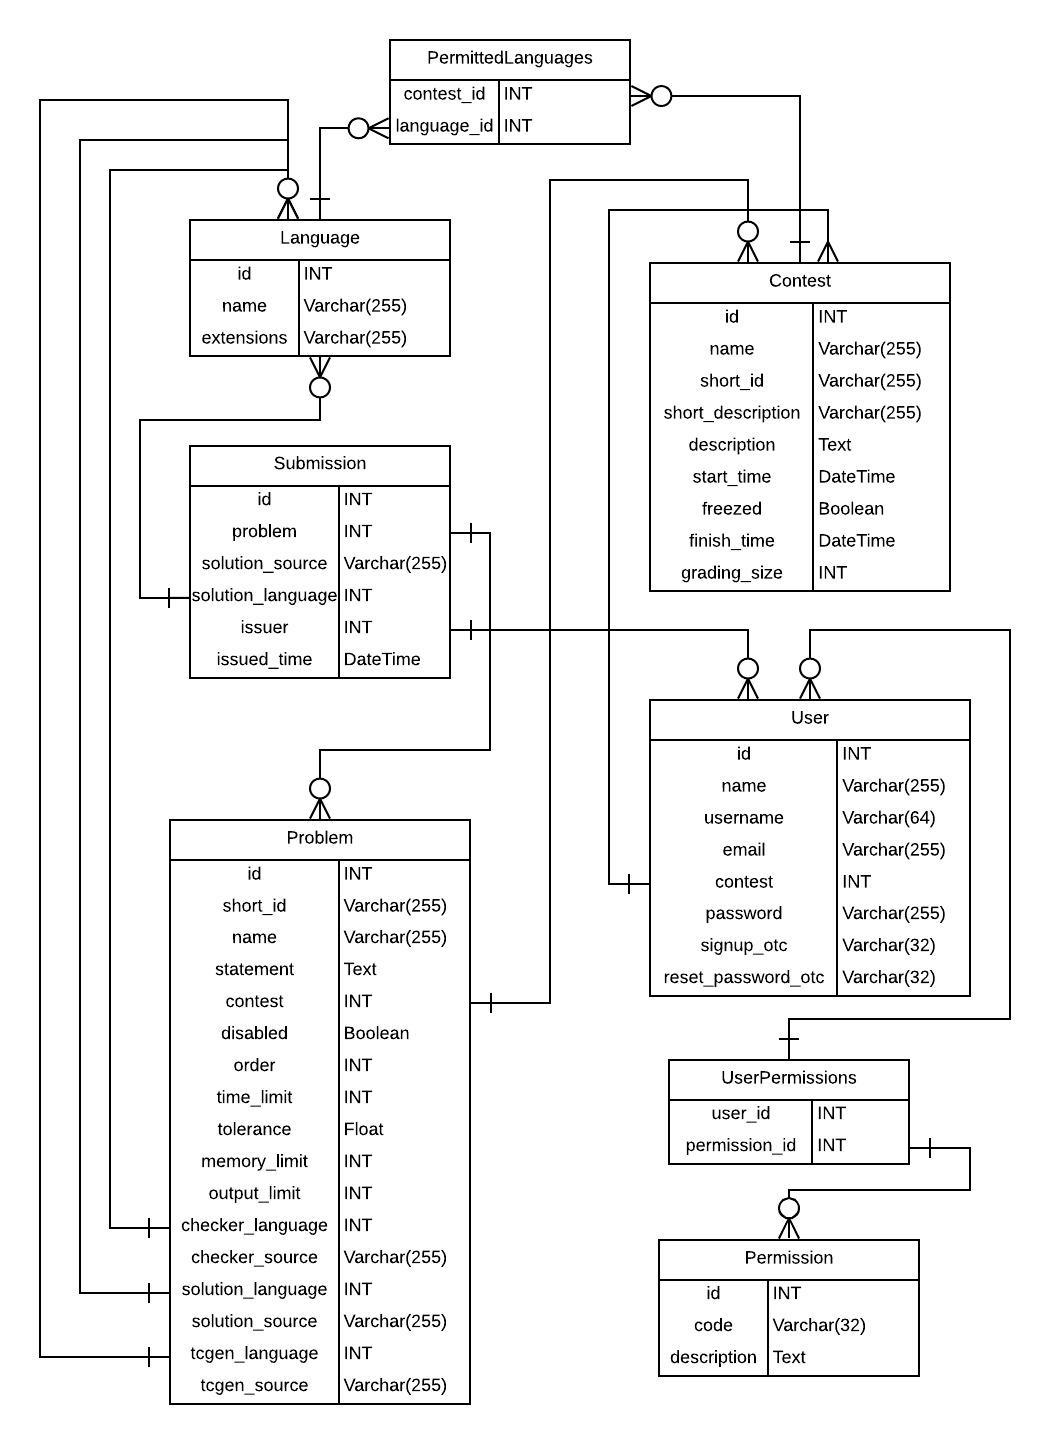
\includegraphics[width=0.8\textwidth]{images/dbschemas}
    \caption{Skema Basis Data Sistem Manajemen Kompetisi}
    \label{fig:dbschemas}
\end{figure}

\par Dalam menjalankan fungsinya, \textit{UGServer} menggunakan sistem manajemen basis data untuk menyimpan informasi terkait kompetisi. Pada saat ini, \textit{UGServer} dapat berjalan menggunakan sistem basis data \textit{Postgresql} atau \textit{SQLite}. \textit{Framework django} memiliki fitur \textit{ORM} yang siap digunakan untuk basis data yang bersifat relasional. Karena adanya fitur tersebut, data lebih mudah untuk diatur menggunakan basis data relasional. Oleh karena itu, pada Tugas Akhir ini penyimpanan data dilakukan menggunakan sistem basis data relasional. Gambar \ref{fig:dbschemas} merupakan skema basis data yang digunakan untuk menyimpan informasi terkait kompetisi.

\subsection{Manajemen Pengguna}

% akun
\par \textit{UGServer} memberikan layanan untuk melakukan manajemen pengguna. Pengguna pada \textit{UGrade} terikat pada suatu kompetisi. Pengguna pada suatu kompetisi tidak dapat mengikuti kompetisi lain. Pengguna yang ingin mengikuti dua buah kompetisi harus membuat dua akun. Pengguna dapat membuat akun dengan cara membuat kompetisi. Ketika seseorang membuat kompetisi, maka sebuah akun akan tercipta sesuai dengan alamat \textit{email} orang tersebut. Selain itu, akun dapat dibuat dengan mengundang orang lain ke dalam kompetisi.

% otentikasi
\par Akun yang pertama kali dibuat hanya mengandung informasi alamat \textit{email} pengguna dan kode untuk otentikasi. Kode tersebut akan dikirim ke \textit{email} pengguna. Hal ini berfungsi sebagai cara untuk mengotentikasi pengguna dengan cara mengotentikasi \textit{email} pengguna. Pengguna kemudian harus memasukkan kode tersebut untuk mengotentikasi dirinya. Pengguna yang telah terotentikasi akan memasukkan informasi mengenai nama lengkap, \textit{username} dan kata sandi. Nama lengkap merupakan nama yang akan ditampilkan pada antar muka kompetisi. \textit{Username} merupakan nama pengguna yang unik untuk setiap kontes dan bersifat mudah untuk dibaca oleh manusia. Setelah melakukan otentikasi \textit{email}, pengguna selanjutnya dapat melakukan otentikasi dengan kombinasi kompetisi yang diikuti, alamat \textit{email} dan kata sandi yang dipilih. 

% emai + username unik untuk setiap kompetisi
\par Setiap pengguna dalam suatu kompetisi memiliki alamat \textit{email} dan \textit{username} yang unik. Dalam dua kompetisi berbeda bisa saja terdapat akun dengan alamat \textit{email} yang sama. Hal ini dikarenakan akun pengguna terikat pada suatu kompetisi sehingga seorang pengguna dapat diidentifikasi dengan menggunakan informasi kompetisi yang diikutinya dan alamat \textit{email} atau \textit{username}-nya.

\begin{figure}[ht!]
    \centering
    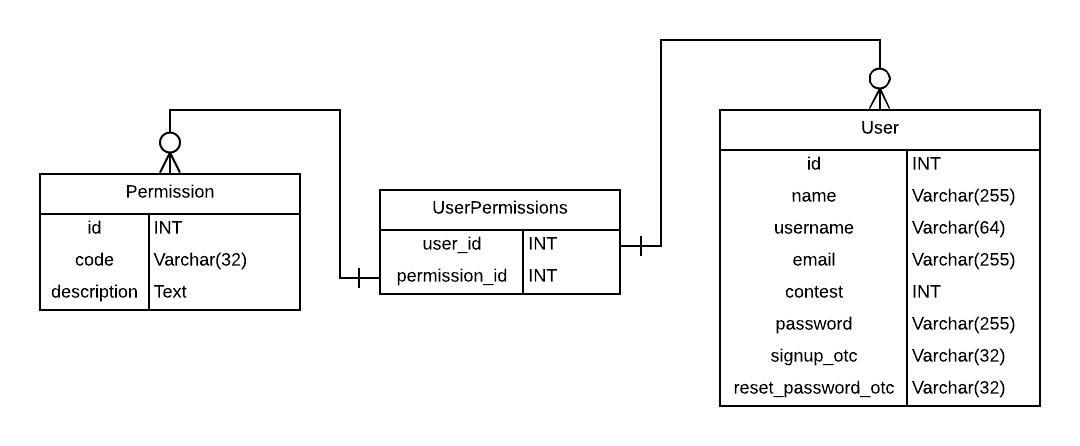
\includegraphics[width=\textwidth]{images/user-schema}
    \caption{Skema Basis Data Sistem Manajemen Pengguna}
    \label{fig:user-schema}
\end{figure}

% user permissions
Pengguna dalam perangkat lunak ini umumnya meliputi juri, peserta dan admin. Perangkat lunak \textit{UGServer} sebenarnya tidak membeda-bedakan pengguna sebagai juri, peserta ataupun admin. Otorisasi dilakukan dengan memberikan label \textit{permission} kepada setiap pengguna yang ada. Setiap pengguna memiliki himpunan \textit{permission} yang menandakan aksi-aksi apa saja yang dapat dilakukan. Pada saati ini, terdapat beberapa \textit{permission} yang mengatur hak akses pengguna yaitu:
\begin{enumerate}
    \item \textit{update:contest}: pengguna dengan \textit{permission} ini dapat mengubah informasi kompetisi.
    \item \textit{create:problems}: pengguna dengan \textit{permission} ini dapat membuat soal baru.
    \item \textit{read:problems}: \textit{permission} ini menandakan seorang pengguna dapat melihat dan membaca soal.
    \item \textit{read:disabledProblems}: beberapa soal dapat ditandai sebagai \textit{disabled} sehingga tidak dapat dibaca oleh pengguna yang tidak memiliki \textit{permission} ini.
    \item \textit{update:problems}: pengguna dengan \textit{permission} ini dapat mengubah informasi soal. Soal yang dapat diubah hanyalah soal yang dapat dilihatnya.
    \item \textit{delete:problems}: sebuah soal dapat dihapus oleh pengguna yang memiliki \textit{permission} ini. Soal yang dapat diubah hanya soal yang dapat dilihat oleh pengguna yang bersangkutan.
    \item \textit{invite:users}: \textit{permission} ini memungkinkan pengguna untuk mengundang pengguna lain.
    \item \textit{update:usersPermissions}: seorang pengguna dapat mengubah \textit{permission} dari pengguna lain jika memiliki \textit{permission} ini.
    \item \textit{delete:users}: pengguna dapat menghapus keanggotaan pengguna lain jika memiliki \textit{permission} ini.
    \item \textit{read:submissions}: dengan \textit{permission} ini, pengguna dapat melihat semua jawaban pengguna lain. \textit{Permission} ini biasanya diberikan untuk juri.
    \item \textit{create:submissions}: \textit{permission} ini memungkinkan pengguna untuk mengirimkan jawabannya. Pengguna tanpa \textit{permission} ini dapat dipandang sebagai seorang penonton.
\end{enumerate}
Pemberian \textit{permission} untuk setiap pengguna bertujuan untuk meningkatkan \textit{granularitas} pada hak akses untuk setiap pengguna. Gambar \ref{fig:user-schema} merupakan skema basis data yang digunakan untuk melakukan manajemen pengguna.

% TODO: further works